\documentclass[]{article}

%opening
\title{A General Guide to CP and Equipment in Lineage 2 Revolution}
\author{Naito - RoyalClub - Vasper Server}
\date{Updated 5 August, 2019}


\usepackage{graphicx}
\graphicspath{{./images/}}

\usepackage[margin=0.5in]{geometry}

\usepackage{array}

\newcommand*\rot{\rotatebox{90}}
%\usepackage[backend=biber]{biblatex}
%\addbibresource{LCG.bib}
\begin{document}

\maketitle

This is a general reference, not a definitive work.
There will be errors, and much of this information is based upon the personal preferences and/or opinions of the author.
Equipment preferences will be based upon the perspective of a PVPer.
PVEers may still find use in this guide, but certain aspects will not apply.

\tableofcontents

\pagebreak
\section{Prioritization}

Your primary focus should be in crafting a UR weapons and armor.
This does not mean that you should completely ignore other areas of CP growth, only that your main focus should always be on crafting new pieces of UR equipment.
The equipment codex provides a good source of CP, so don't think that you can stop crafting UR sets once you are done with your PVP gear.

In general, your priorities should be as follows
\begin{enumerate}
	\item Crafting UR equipment
	\item Agathion
	\item Elixirs
	\item Mount Equipment (support only)
	\item Talisman
	\item Enhancements (only this low due to difficulty in acquiring materials)
	\item Soul Crystals 
	\item Everything Else.
\end{enumerate}

2-5 are fairly close together in priority, while the gap between 5 and 6 is very wide.
\section{Your Equipment}

Typically, your PVP set will be your primary focus, however, you will reach a point where you will need to shift focus toward your other equipment sets.

PVP equipment has a blue background, PVE equipm

Equipment Set Priorities
\begin{enumerate}
	\item PVP - Your primary set and mandatory for PVP.
	\item Aegis (Magic set) - Useful for leveling from level 80+, and a necessity for both nightmare rifts and Temple Garden.
	\item Draconic - Useful for leveling 320+ and a necessity for Temple of Dragon Hearts rift.
	\item Human - Useful for leveling 362+ and a necessity for Spore Epicenter rift.
	\item Elite set - Useful in rifts, as well in dungeon grinding.
	\item Normal weapon - Very useful for field farming and Summoning Circle.
	\item Boss set - The weapon is more useful than the armor, but both are fairly easy to craft.

\end{enumerate}

\subsection{Equipment Substats}

Before upgrading any piece of equipment to SR, it is a good idea to take the time to think about its substats.
Typically, you will want to get at least 2/3 of your equipment's substats to be from the top 3 of the following tables.
If you are short of red gems, rerolling substats while the piece is still R grade is a good idea, as the cost at R grade is only 50 gems compared to 100 gems at SR.

%\includegraphics[width=\textwidth]{substats.png} %Substats table
\begin{center}
	\textbf{PVE Substats}\\
\begin{tabular}{|c|c|c|c|c|c|}
	\hline 
	%\multicolumn{6}{|c|}{\textbf{PVE Substats}} \\ 
%	\hline 
	\rule[-1ex]{0pt}{2.5ex} Equipment & \multicolumn{3}{c|}{Top 3 Options} &\multicolumn{2}{c|}{Additional Options} \\ 
	\hline 
	\rule[-1ex]{0pt}{2.5ex} Weapon & Atk. Speed & Crit Rate & HP Drain & P. Atk/M. Atk & Crit Dmg. \\ 
%	\hline 
	\rule[-1ex]{0pt}{2.5ex} Helmet & HP Drain & P. Def & M. Def & Penetration & Evasion \\ 
%	\hline 
	\rule[-1ex]{0pt}{2.5ex} Armor & P. Def & M. Def & Evasion & Resilience & Move Speed \\ 
%	\hline 
	\rule[-1ex]{0pt}{2.5ex} Gloves & P. Atk/M. Atk & Penetration & Evasion & MP Cost Reduction$*$ & - \\ 
%	\hline 
	\rule[-1ex]{0pt}{2.5ex} Boots & Atk. Speed & P. Atk/M. Atk & Evasion & Resilience & Move Speed \\ 
%	\hline 
	\rule[-1ex]{0pt}{2.5ex} Necklace & Atk. Speed & HP Drain & P. Def/M. Def & Skill CD Reduction$*$ & Accuracy \\ 
%	\hline 
	\rule[-1ex]{0pt}{2.5ex} Earrings & HP Drain & Penetration & Move Speed & MP Cost Reduction$*$ & - \\ 
%	\hline 
	\rule[-1ex]{0pt}{2.5ex} Rings & HP Drain & Crit Rate & P. Atk/M. Atk & Crit Resist & - \\ 
	\hline 
\end{tabular}
\\ 
$*$Useful if you plan on using skills while AFK farming
\\
%\\
\textbf{PVP Substats}
\begin{tabular}{|c|c|c|c|c|c|c|}
	\hline 
	%\multicolumn{7}{|c|}{\textbf{PVP Substats}} \\ 
	%\hline 
	Equipment & \multicolumn{3}{c|}{Top 3 Options} & \multicolumn{3}{c|}{Additional Options}\\ 
	\hline 
	Weapon & Atk. Speed & Crit Rate & Crit Dmg & P. Atk/M. Atk & Penetration & - \\ 
%	\hline 
	Helmet & ASR$\star$ & P. Def & M. Def & Penetration & Evasion & - \\ 
%	\hline 
	Armor & P. Def & M. Def & Move Speed & Evasion & Resilience & - \\ 
%	\hline 
	Gloves & P. Atk/M. Atk & Penetration & Evasion & MP Cost Reduction$*$ & - & - \\ 
%	\hline 
	Boots & Atk. Speed & P. Atk/M. Atk & Move Speed & Evasion & Resilience & MP Cost$*$ \\ 
%	\hline 
	Necklace & ASR$\star$ & Atk. Speed & Resilience & Crit Resist & M. Def/P. Def & Skill CD \\ 
%	\hline 
	Earrings & ASR$\star$ & Penetration & Move Speed & MP Cost Reduction$*$ & - & - \\ 
%	\hline 
	Rings & ASR$\star$ & Crit Rate & P. Atk/M. Atk & Crit Resist & Crit Dmg. & - \\ 
	\hline 
\end{tabular} 

$\star$ Abnormal Status Resistance\\
$*$Useful for Healers
\end{center}
These tables are open to your personal preferences or class needs. 
For example, tanks and healers may want to exchange HP drain for DPS substats on their non-weapon PVE gear to improve their farming efficiency
Melee classes may also find movement speed useful in PVE to decrease downtime as they move from mob to mob.

Due to the limited usage of boss armor, it is not a bad idea to roll Exp. Gain Increase Rate on all four pieces of armor. Equipping these pieces during a clan hall fire can increase your experience gains substantially.
\subsection{Selecting Accessories}

With the introduction of auxiliary accessory slots and secondary attributes, selecting an accessory set to utilize and develop has become even more complicated.
Every character will receive an SR Nassen set, which is a fantastic option for either your primary or auxiliary accessory slots.
For selecting a secondary set, your first thought should be on whether or not your goal is to take part in competitive battlefield PVP (castle and fortress sieges, 3v3, and so on).
If so, then the Hero set is a great option to pair with your existing accessories as its attributes give a significant competitive edge in battlefield PVP.
If the battlefield is not your cup of tea, then take a glance at the following information to help you in finding your accessory sets.
\\
\begin{center}
	\textbf{Accessory Attributes}
\end{center}
$\bullet$ Elven: Stun Resistance, Accuracy\\
$\bullet$ Moonstone: M. Def, \% M. Def Increase\\
$\bullet$ Phoenix: Slow Resistance, Max HP\\
$\bullet$ Black Ore: Critical Resistance, Decreased Damage from Monsters\\
$\bullet$ Nassen: Speed Increase, Evasion\\
$\bullet$ Arbol: Increase Combo Duration, Normal Attack Damage Increase\\
$\bullet$ Hero: Attack Speed$*$, Normal and Rare Skill Damage Decrease$*$, Abnormal Status Resist$*$\\
$*$Only active while in a battlefield

%\includegraphics[width=\textwidth]{Accessory_subs.png}
\pagebreak
\begin{center}
	\textbf{Accessory Substat Values at SR Grade}

\begin{tabular}{|cc|l|l|l|l|l|l|l|l|l|l|l|l|l|l|l|}
	\hline 
	\rule[-1ex]{0pt}{2.5ex} Set & Piece & \rot{P. Atk} & \rot{M. Atk} & \rot{Atk. Spd.} & \rot{Crit Dmg.} & \rot{Crit Rate} & \rot{Crit Res.} & \rot{P. Def} & \rot{M. Def} & \rot{Accuracy} & \rot{Max HP} & \rot{Max MP} & \rot{Move Spd.} & \rot{ASR} & \rot{Penetration } & \rot{Resilience} \\ 
	\hline 
	\rule[-1ex]{0pt}{2.5ex} Arbol & Necklace &  &  & 432 &  &  & 761 & 508 & 508 & 365 & 358 & 341 &  & 360 &  & 451 \\ 
%	\hline 
	\rule[-1ex]{0pt}{2.5ex} Arbol & Earring &  &  &  &  &  & 761 &  &  & 365 & 358 & 341 & 432 & 360 & 338 &  \\ 
%	\hline 
	\rule[-1ex]{0pt}{2.5ex} Arbol & Ring & 396 & 396 &  & 356 & 678 & 761 &  &  & 731 & 358 & 341 &  & 360 &  & 451 \\ 
	\hline 
	\rule[-1ex]{0pt}{2.5ex} Black Ore & Necklace &  &  & 345 &  &  & 761 & 406 & 406 & 346 & 273 & 307 &  & 324 &  & 405 \\ 
%	\hline 
	\rule[-1ex]{0pt}{2.5ex} Black Ore & Earring &  &  &  &  &  & 761 &  &  & 346 & 273 & 307 & 345 & 324 & 304 &  \\ 
%	\hline 
	\rule[-1ex]{0pt}{2.5ex} Black Ore & Ring & 302 & 302 &  & 356 & 645 & 761 &  &  & 692 & 273 & 307 &  & 324 &  & 405 \\ 
	\hline 
	\rule[-1ex]{0pt}{2.5ex} Elven & Necklace &  &  & 345 &  &  & 608 & 406 & 406 & 308 & 273 & 341 &  & 324 &  & 360 \\ 
%	\hline 
	\rule[-1ex]{0pt}{2.5ex} Elven & Earring &  &  &  &  &  & 308 &  &  & 308 & 273 & 341 & 345 & 324 & 270 &  \\ 
%	\hline 
	\rule[-1ex]{0pt}{2.5ex} Elven & Ring & 377 & 377 &  & 285 & 516 & 608 &  &  & 616 & 273 & 341 &  & 324 &  & 360 \\ 
	\hline 
	\rule[-1ex]{0pt}{2.5ex} Moonstone & Necklace &  &  & 345 &  & 608 & 608 & 508 & 308 & 341 & 273 &  & 324 &  & 360 &  \\ 
%	\hline 
	\rule[-1ex]{0pt}{2.5ex} Moonstone & Earring &  &  &  &  &  & 608 &  &  & 308 & 341 & 273 & 345 & 324 & 270 &  \\ 
%	\hline 
	\rule[-1ex]{0pt}{2.5ex} Moonstone & Ring & 302 & 302 &  & 285 & 516 & 608 &  &  & 616 & 341 & 273 &  & 324 &  & 360 \\ 
	\hline 
	\rule[-1ex]{0pt}{2.5ex} Nassen & Necklace &  &  & 432 &  &  & 799 & 533 & 533 & 404 & 341 & 358 &  & 360 &  & 451 \\ 
%	\hline 
	\rule[-1ex]{0pt}{2.5ex} Nassen & Earring &  &  &  &  &  & 799 &  &  & 404 & 341 & 358 & 432 & 360 & 338 &  \\ 
%	\hline 
	\rule[-1ex]{0pt}{2.5ex} Nassen & Ring & 377 & 377 &  & 356 & 645 & 799 &  &  & 808 & 341 & 358 &  & 360 &  & 451 \\ 
	\hline 
	\rule[-1ex]{0pt}{2.5ex} Phoenix & Necklace &  &  & 432 &  &  & 685 & 406 & 406 & 308 & 273 & 273 &  & 324 &  & 405 \\ 
%	\hline 
	\rule[-1ex]{0pt}{2.5ex} Phoenix & Earring &  &  &  &  &  & 685 &  &  & 308 & 273 & 273 & 432 & 324 & 304 &  \\ 
%	\hline 
	\rule[-1ex]{0pt}{2.5ex} Phoenix & Ring & 302 & 302 &  & 321 & 581 & 685 &  &  & 616 & 273 & 273 &  & 324 &  & 405 \\ 
	\hline 
	\rule[-1ex]{0pt}{2.5ex} Hero & Necklace &  &  & 345 &  &  & 685 & 406 & 406 & 308 & 273 & 341 &  & 324 &  & 383 \\ 
%	\hline 
	\rule[-1ex]{0pt}{2.5ex} Hero & Earring &  &  &  &  &  & 685 &  &  & 308 & 273 & 341 & 345 & 324 & 287 &  \\ 
%	\hline 
	\rule[-1ex]{0pt}{2.5ex} Hero & Ring & 377 & 377 &  & 285 & 581 & 685 &  &  & 616 & 273 & 341 &  & 324 &  & 383 \\ 
	\hline 
\end{tabular} 
\end{center}

For auxiliary sets, you will only receive 30\% of the stats and CP from that set, so remember to factor that in while looking at the accessory substats table.

For most classes, a combination of Elven and Nassen will be your best bet.
For PVPers, either Elven/Hero or Nassen/Hero are the most commonly used combinations.
Healers may favor a Moonstone/Nassen choice in order to maximize their survivability .
A phoenix set is not a bad option for tanks or other high defense melee classes in PVP, as the slow resist and HP increase can help in keeping you alive while closing in on your target.
Black ore provides a good mix of PVP and PVE attributes.
Arbol's increased normal damage attribute and high substat values aren't enough to overcome the low usefulness of Arbol's other attribute - there are better options for PVPers and PVEers.

\subsection{Equipment Attribute Level}

Increasing your gear attributes is a decent way to increase your CP.
Your CP will grow with every increase in attribute level, and you will satisfy a requirement in the equipment codex for every even attribute level (2,4,6, and so on).

When and how you level up an item's attribute level depends upon many factors,

$\bullet$ Prioritize weapon attributes before armor, and prioritize your weapons and armor before your accessories.

$\bullet$ For Weapons, PVP\textgreater Magic $\ge$ Draconic \textgreater Elite \textgreater Boss \textgreater Normal

$\bullet$ For armor, PVP \textgreater Magic $\ge$ Draconic $\ge$ Elite $\gg$ Boss

Use attribute stones to level your rare equipment and S/R equipment for your non-rare items (including accessories).
SR equipment can be used to for leveing attributes, but this should only be done if you have fully limit broken the equipment (see the next subsection for information on limit breaking).

Start with S tier equipment or stones on the off-chance that they suceed.
If the item fails to increase in attribute level, use an R tier item.
If the R tier item fails, use more S tier items until your attribute level increases, at which point you can repeat this pathway.

\pagebreak
\begin{center}
	\textbf{Attribute Enhancement Odds}\\
\begin{tabular}{|c|c|c|}
	\hline 
	Item & Odds of Success & Bonus Upon Failure \\ 	\hline 
	S Attribute Stone & 8\% & 10\% \\ 	 
	R Attribute Stone & 25\% & 25\% \\ 	 
	SR Attribute Stone & 100\% & N/A \\ 	 
	UR Attribute Stone & 100\% - Adds 2 levels & N/A \\ 	 
	S Equipment & 10\% & 3\% \\ 	 
	R Equipment & 25\% & 10\% \\ 	 
	SR Equipment & 100\% & N/A \\ 	\hline 
\end{tabular} 
\end{center}

Bonus odds do not carry over if you use an SR or UR stone, or SR equipment, so be sure to double check before using those items.

\subsection{Equipment Limit Breaking}

Limit breaking is a fantastic way to increase your CP, but just as with attribute levels, how and when you should limit break has many factors involved.

$\bullet$ Rare Equipment - This should be your priority for limit breaking.
Save any limit break stones for your rare equipment
Rare equipment pieces should only be used for limit breaking if you have already elevated that piece (or pieces in the case of armor) to UR, otherwise that rare equipment should be used for salvage (see 2.4.1 for more information on salvage).

$\bullet$ Elite/Boss/Normal Equipment - Use SR tier items from this group as fodder for attribute level before you work on limit breaking, as the increase or decrease in damage from the attribute is far more valuable than the slight bump in stats from limit breaking.

$\bullet$ Accessories - This will slightly depend upon your accessory set, however, the general view is that accessories should be limit broken before you start to attribute enhance. 
Typically, you will want to start with rings, followed by your necklace, then finish up with earrings.
If you PVP set is fully limit broken, then any limit break stones can go toward your accessories.

\begin{center}
	\textbf{Limit Breaking Odds}\\
	\begin{tabular}{|c|c|c|}
		\hline 
		Item & Odds of Success & Bonus Upon Failure \\ 
		\hline 
		SR Equipment & 50\% & 25\% \\ 
%		\hline 
		SR Limit Break Stone & 50\% & 25\% \\ 
%		\hline 
		UR Limit Break Stone & 100\% & N/A \\ 
		\hline 
	\end{tabular} 
\end{center}

Just as with limit breaking, bonus odds do not carry over so be sure to double check everything before attempting a limit break.

\subsection{Crafting UR Equipment}

Crafting UR equipment is going to be your main focus in L2R.
The materials needed to craft any piece of UR equipment are significant, and can take a while to gather.
The upside to this is that UR equipment is perhaps the largest CP boost available in the game, with most pieces gaining between 50k and 100k CP at UR 30+ from SR 30+.
Any piece of level 30 or higher SR equipment is eligible for UR crafting.

In general, you will want to focus on getting a set of UR PVP gear first, followed by your aegis set then your draconic set.
With the exception of upgrade stones, you will easily accumulate enough materials to craft non-rare sets while building your rare UR's.
Of the non-rares, your elite set should be a priority as it makes a significant difference in rifts and allows you to grind in less crowded areas.
The boss set and normal weapon are fairly low priority and can be crafted later (Normal weapon can be slightly more useful to UR than boss, as it improves field grinding).

Accessories will take a while to grind, so you can passively accumulate materials for your accessories while grinding for your other UR pieces.

\subsubsection{Weapons and Armor}

For weapons and armor, you will need the following,\\
\begin{center}
	\textbf{Materials Required to Craft UR Equipment}\\
	\begin{tabular}{|c|c|c|c|c|}
		\hline 
		UR Materials & Rare Weapon & Non-Rare Weapon & Rare Armor & Non-Rare Armor \\ 
		\hline 
		Recipes (scaps per recipe, fragments per recipe) & 15 (5000, 30) & 15 (1500,10) & 10 (5000, 30) & 10 (1500, 10) \\ 
%		\hline 
		Scrap & 5000 & 5000 & 5000 & 5000 \\ 
%		\hline 
		Radiant Upgrade Stones & 10 Weapon & 10 Weapon & 10 Armor & 10 Armor \\ 
%		\hline 
		Material & 250 Rare & 250 Non-rare & 150 Rare & 150 Non-rare \\ 
		\hline 
	\end{tabular} 
\end{center}

With the exception of radiant upgrade stones, most of this equipment can come from salvaging.
With salvaging, you will want to do A+A combines with the goal of obtaining rare weapons or armor.
With the rare pieces, they should be upgraded to SR before attempting to salvage, while any piece of non-rare equipment at S or R grade can be turned in to immediate salvage fodder (you can do S+S combines with non-rares but the cost is much higher than A+A).

\begin{center}
	\textbf{Equipment Salvage per Grade Tier}\\
	\begin{tabular}{|c|c|c|c|}
		\hline 
		Tier (grade) & Scrap & Recipe Fragments & Materials (Normal, Rare) \\ 
		\hline 
		SR (rare) & 1208 & 7 & 30, 30 \\ 
%		\hline 
		SR (non-rare) & 805 & 3 & 30, 7 \\ 
%		\hline 
		R (non-rare) & 350 & 0 & 8, 2 \\ 
%		\hline 
		S (non-rare) & 150 & 0 & 2, 0 \\ 
		\hline 
	\end{tabular} 
\end{center}

For recipe fragments, your best bet is to farm Zaken and Guilotine world bosses (Section 4 for more information), purchase the daily recipe fragment from the clan shop, purchase the Honor Summon Box (15 coins) and 10 Grade UR Accessory of the Hero Material Box (150 coins) from the Honorable Battlefield shop, and to keep an eye out for events that hand out fragments.
Fragments are one of the limiting components for crafting UR weapons and armor, so you will want to farm them on a consistent basis.

Scrap drops randomly while farming, and is fairly easy to get from salvage.
Scrap is also obtained through Temple Garden, the Honorable Battlefield shop (in bundles or as unconfirmed), and is common in events.

Random materials boxes can be obtained through rifts, though these boxes are more likely to give normal materials than rares, through events (often as selection boxes), or in the Honor Summon Box.
Your best bet is to salvage equipment.

\subsubsection{Accessories}

UR accessories are currently very time intensive, and it's best to passively grind the materials until you have hit the high 2 millions in CP.

\begin{center}
	\textbf{Materials Needed to Craft a UR Accessory}\\
	\begin{tabular}{|c|c|c|c|c|}
		\hline 
		Recipes* (scrap per) & Radiant Upgrade Stones & Accessory Scrap & Gold Ingots** & Beads*** \\ 
		\hline 
		10 (1500) & 10 & 3000 & 150 & 150 \\ 
		\hline 
	\end{tabular} 

\end{center}
*Recipes are unique to the accessory set (Nassen requires Nassen recipes).\\
**The Hero set requires its own set of ingots, which are obtainable from the Honorable Battlefield '10 UR' bundles or salvage, all other accessories use normal Gold Ingots.\\
***Beads are unique to each accessory set, however, the Hero set beads can only be obtained via the '10 UR' bundles in the Honorable Battlefield shop.\\

\begin{center}
	\textbf{Accessory Salvage per Grade Tier}\\
	\begin{tabular}{|c|c|c|c|}
		\hline 
		Tier & Recipe Fragments & Scrap & Gold Ingots \\ 
		\hline 
		SR & 3 & 805 & 30 \\ 
%		\hline 
		R & 0 & 350 & 8 \\ 
%		\hline 
		S & 0 & 150 & 2 \\ 
%		\hline 
		SR Hero & 7 & 1200 & 30 \\
%		\hline
		R Hero & 0 & 525 & 8 \\
%		\hline
		S Hero & 0 & 225& 2 \\
		\hline
	\end{tabular}  
\end{center}

Scrap is best obtained from unconfirmed scrap and salvage, as other methods are low yield.
The unconfirmed scrap from SR Temple Garden runs should yield about 100-150 accessory scrap upon usage, which equates to a recipe every 10-15 days.

Gold ingots are fairly easy to obtain from just salvaging SR accessories, since any set will give them.

Beads are the limiting factor in UR accessory crafting.
They can be obtain via two ways: directly as drops, or indirectly from unconfirmed beads (dropped from Nightmare rifts, field farming).
Your best bet is to field farm mobs which drop your bead of choice (see the monster info tab on the in-game map) while using a flute.
This method will result in unconfirmed bead drops and beads of your preferences.
You can turn beads from unwanted sets in to uncomfirmed beads at the cost of 30 accessory scrap per bead, so do not sell or discard those unwanted beads!

\subsection{Soul Crystals}

Souls crystals are a fairly small source of CP, and can be quite expensive to upgrade.
Using S grade crystals, it will cost approximately 3.2 million adena to upgrade one R crystal to SR.

Typically, you will want to upgrade your attack, defense, and HP crystals first, followed by crit rate and crit resist, then evasion and accuracy.
Penetration and resilience crystal are very hard to come by (penetration in particular), so it is a good idea to use any R/SR soul crystal selection boxes on these two soul crystals.

There are special crystals from the Batman and Monster Strike events that provide higher stats, and those should be used in your main gear set.

\subsection{Equipment Enhancement}

Enhancing equipment is the worst part of Lineage 2 Revolution.
Many people have strategies for equipment enhancing, but most of those are superstition.
There isn't a surefire method to game the system, it's really just based upon luck.
A good rule of thumb is to stop enhancing after 3 failures (just close the inventory and do something else), and to avoid going on tilt and start spamming enhances after a frustrating failure.

Your first goal is to get a piece of +20, which is the easiest step in enhancing.
If you have an abundance of blessed scrolls, then feel free to use a few at +15 or higher in an effort to save some adena, but don't waste them!


Once you have hit +20, you will have several pathways to +30 available to you, but these two are the more common.\\
\begin{center}
	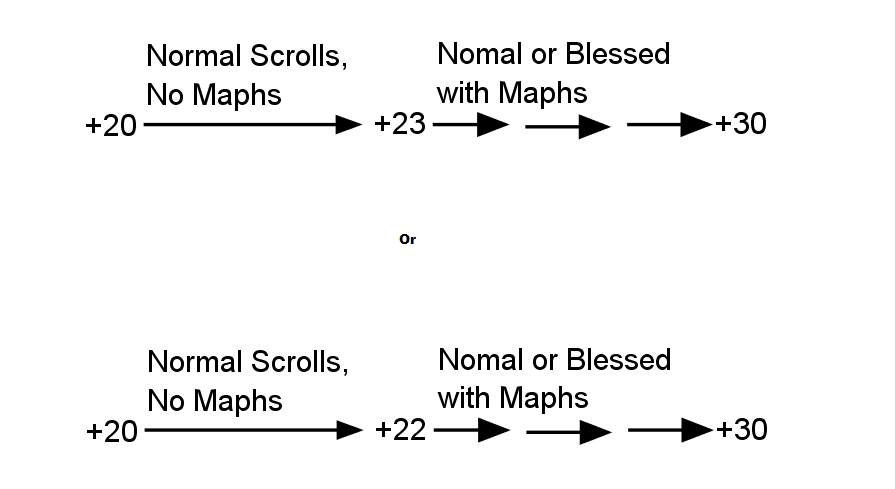
\includegraphics[width=0.7\linewidth]{EnhPath}
\end{center}

 Some players find it best to attempt an unprotected blessed enhancement at +23 or +22 (no maphs) in an effort to hit +25, but this can prove costly to your CP as failure is more likely than success.
 
 If you happen to get stuck at +29 or +28, you may consider enhancing without using maphs until you either max your enhancement or you reach +27.
 The CP loss from failing at these levels may be demoralizing, but saving your maphs for other pieces of equipment will help in the long run.
 If you opt to use this strategy, remember not to go below +27.
 
 Maphr's Protection - often just called 'maphs' - are going to be your bottleneck for enhancing.
 Failed enhances above +10 will give fragments, and this is your best bet for obtaining maphs.
 A good idea is to have a piece of equipment that is used only as a method for farming maph fragments.
 The adena cost can run fairly high using this method of maph farming, but it is a reliable and easy way to farm maphs.

\section{Mounts}

Mounts are an often overlooked method for increasing your CP.
You will want to focus solely on your 'support' mount, as the other mounts will gain very small amounts of CP with these methods.

For equipment, there are only two substats that you need to care about: crit resist (for boots and saddle) and crit rate (for visor and armor).
These two substats provide the most CP for those pieces.
For boots and saddle, it is best to just level a new piece of equipment with the desired substat rather than using red gems to reroll existing equipment - save those red gems for rerolling visor and armor, as those pieces are hard to come by!

Mount equipment enhancement has no failure penalty and a fairly low cost, so feel free to enhance your mount gear whenever.
Mount equipment enhancement is one of the easiest and most cost effective ways to increase your CP right now.
Mount enhancement scrolls can be found in the higher levels of the daily dungeon.

\section{Runes}

Runes can be an okay source of CP but they get very expensive very quickly.
It is best to set a budget - say 250k adena per day - and chip away at your runes overtime.
With how random number generation works in this game (it favors runs of successes or failures), if you happen to fail more than 3-5 times in a row, stop and do something else.


\section{Elixirs}

Elixirs are a decent and dependable source of CP.
They can get expensive, but there is no risk of failure like with runes.

To start with, make sure to purchase the Garden cloak from the shop and make it a priority to level (at level 30, you basically get 10 free herbs).
Hunt for the large flowers, as they give double, and purchase elixirs from the fortress shop if your clan holds a fortress.

Level up attack, then defense or HP (preference), and leave MP for last as it gives the lowest CP.
For the new herbs, crit rate and crit resist before evasion and accuracy.

\section{Monster Codex}

There isn't a lot to say about monster codex other than it is the easiest way to increase your CP.
Do not neglect your monster codex!

Mobs that are within 4 levels of you will provide the highest drop rates, but this really only matters in field farming or elite dungeon farming.

It is a good idea to be watching the public channel for summoning stones while you are playing, as these are fast and free methods to farm the monster codex.
Save your summoning stones for core buffs and/or core pot parties (buff and pots stack!), as the drop rate from having all 5 members with a buff is much, much higher than it is with just you and your buff.

Save lower level summoning stones for the end of buff runs;
if you have 5 minutes left on a core pot, you can use that time to summon some low level dungeon mobs to farm A grade cores for dust.

In general, prioritize the codex as follows\\
\begin{enumerate}
	\item Attack
	\item Defense
	\item HP
	\item Crit Rate, Penetration
	\item Crit Resist, Resilience
	\item Accuracy, Evasion, MP

\end{enumerate}
Of course, these are open to class necessities, such as MP for healers or evasion for daggers having higher priorities than for other classes.

Zaken tickets can be obtained from the magical monsters in Forest of Secrets Understory, while Guillotine tickets can be farmed from any mob in the Ivory Tower Laboratory. 
Guillotine spawns occur once every 12 hours and you will have about 30 minutes to 1 hour to enter the boss arena before the window closes.
You may kill Guilotine only once per day.
Zaken spawns once per day (one hour after Guilotine's second spawn) and you will have only one shot to kill him.
The most effective strategy to enter Zaken's arena is to enter the portal about 30 seconds before spawn, hold the enter button down and release it when the "Zaken has spawned" message appears in the chat window.


World bosses spawn every four hours may be killed after every spawn.
If the boss is too strong for you, try joining a party and standing outside of the boss's attack radius.

\pagebreak
\section{Agathion}
Agathion are the pets that follow people around.
They are a decent source of CP, but they run on the expensive side.

You can obtain agathion souls, which are used to summon an agathion, or agathion charms, from the Agathion summon box for 80 red gems in the common shop. 

There are 7 tiers of agathion: C-SR and SR rare.
You can combine 3 agathion souls of the same tier to create 1 random agathion soul of the next tier.
However, combining 3 SR souls does not mean that you will obtain an SR rare, only that you will have a chance to obtain one.

You can only summon one agathion of any tier at one time.
Any strengthening done to a lower tiered agathion will carry over to a higher tier one.


\begin{center}
\textbf{Agathion Stats and Charm Special Effects}
\begin{tabular}{|c|c|c|}
	\hline 
	Agathion & Stats & Rare Charm Effect \\ 
	\hline 
	Little Demon & Crit Rate, Penetration, Attack & - \\ 
%	\hline 
	Little Angel & Resilience, Crit Res, Defense & - \\ 
%	\hline 
	Royal Hamstar & Evasion, Resilience, Attack & - \\ 
%	\hline 
	Jiangshi & Evasion, Max HP, Defense & Increased exp rate \\ 
%	\hline 
	Pegasus & Attack, Max MP, Crit Rate & Reduced Revival time in castle siege \\ 
%	\hline 
	Valakas & Defense, Max HP Resilience & Increases the CV removed from Crosses of Repentance \\ 
%	\hline 
	Funguy & Defense, Max HP, Resilience & Increases adena acquisition rate \\ 
%	\hline 
	Rudolph & Defense, Evasion, Crit Res & Increases hot time in Elite Dungeons \\ 
	\hline 
\end{tabular} 
\\

\end{center}

Agathion can be strengthened to increase their substats.
There are two methods to accomplish this: normal strengthening (30k adena) or high-grade strengthening (300 reds).
Normal strengthening has a chance to decrease substats, while high-grade strengthening can only increase.
It's best to avoid high-grade strengthening due to the high gem cost.

Charms are equipment for the agathions.
Charms are unique to each agathion, and up to 6 charms may be equipped to any summoned agathion.
Charm stats are determined randomly, and once equipped, charms cannot be removed.
If you wish to equip a new charm while an existing charm is in place, then the existing charm will be deleted.
Rare charms may only be equipped on rare agathion.


\section{Talisman}

At first glance, the talisman system can be overwhelming
You have two different codices, an equipment system, a crafting system, and a variety of attributes and statistics to keep track of.
The steep learning curve may seem daunting, but the talisman system is actually fairly straightforward and it presents a good opportunity for both CP growth as well as improved PVP and farming ability.

To start with, let's focus on the talisman itself.
There are two types: attribute talisman and normal talisman.
You may equip 1 attribute talisman and 7 normal talismans at once.
You can equip different talismans to your various battle decks, allowing for a lot of customization.
Within the talisman types exist several subtypes which are reflected by their color.
Talisman tiers generally relate to their innate effects, with higher tiers having more effects (and better effects) than lower tiers.

\begin{center}
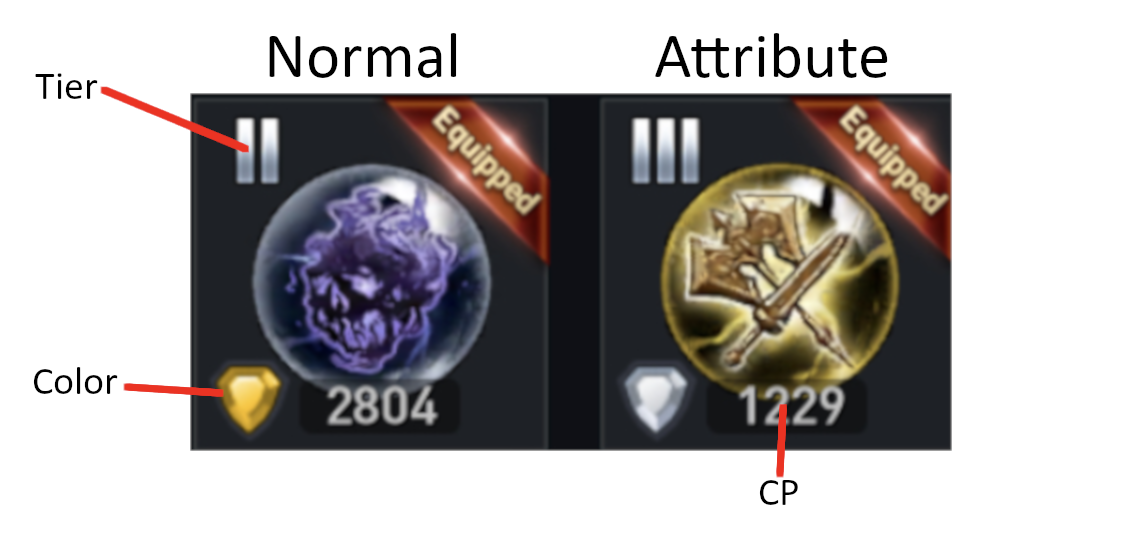
\includegraphics{talis2}
\end{center}

In addition to their innate effects, talisman will have random effects.
These random effects are typically similar to a talisman's innate effects, but the quantity (1-6) and type are randomized.
Typically, attribute talisman that give bonus damage to specific monster types will have randomized effects that provide additional bonus damage and only 2 options for random effects, while attribute talisman that have +speed or +stun resistance will have random effects similar to the attributes on accessory (stun resist, knockdown resist, speed, and so on) and will have about 6 random effect options.
For normal talisman, you will see several options and their specific effects are identical to what you'd expect to see in the innate effects (crit res, pen, rare skill dmg decrease, and so on).
 
\pagebreak
Note: Shop only refers to a talisman only being found in the monster shop;
in addition to the listed drop location, talisman may be found in item boxes.
\begin{center}
	\textbf{Blue Talisman}
	\begin{tabular}{|>{\centering}m{4cm}|c|>{\centering}m{4cm}|>{\centering}m{3cm}|c|c|}
		\hline 
		Name & Tier & Innate Effects & Drop Location & Type & Codex (N,C)\\ 
		\hline 
		Guillotine's Iron Armor Fragment & II & Res, Rare Skill Dmg Decrease & Guillotine & Normal & N \\ 
%		\hline 
		Hunter's Protection & I & P. Def. & Shop Only & Normal & N \\ 
%		\hline 
		Voice of Avento & II & P. Def, Max HP & Field & Normal & N \\ 
%		\hline 
		Lord's Honor & III & Evasion, PVP Crit Dmg Decrease & Castle Siege & Normal & N \\ 
%		\hline 
		Key of Aden & IV & Evasion, Accuracy, Max MP & Field & Normal & N\\ 
%		\hline 
		Dragon Hunter's Crown & III & Bonus Dmg to Draconian & Field & Attribute & N\\ 
%		\hline 
		Warrior's Will & III & Crit Res Rate Increase & Castle Siege, Elite & Attribute & N\\ 
%		\hline 
		Promise of Pixies & III & Max HP, Rare Skill Dmg Decrease & Bind & Normal & C\\
		
		Order of Schuttgart & II & Evasion, Res & Field & Normal & C\\
		
		Hunter's Token & I & Rare Skill Dmg Decrease & Shop Only & Normal & C\\
		
		Blessing of Pixies & II & Bonus Dmg to Normal & Bind & Attribute & C\\
		
		Fate of Schuttgart & II & Max MP, PVP Crit Dmg Decrease & Field & Normal & C\\
		
		\hline
	\end{tabular} 


\textbf{Red Talisman}

\begin{tabular}{|>{\centering}m{4cm}|c|>{\centering}m{4cm}|>{\centering}m{3cm}|c|c|}
	\hline 
	Name & Tier & Innate Effects & Drop Location & Type & Codex (N,C) \\ 
	\hline 
	Luminosity of the Battlefield & I & Rare Skill Dmg Decrese & Honorable Battlefield & Normal& N \\ 
%	\hline 
	Glory of Hunters & I & Resilience & Shop Only & Normal&N \\ 
%	\hline 
	Roland's Mushroom & IV & Evasion, Penetration, Resillience & Spore Epicenter & Normal&N \\ 
%	\hline 
	Eternal Honor & II & Bonus Dmg to Elite & Honorable Battlefield & Attribute&N \\ 
%	\hline 
	Sun Talisman & III & Stun and Knockdown Rest Rate & Castle Siege, Elite & Attribute & N\\ 
%	\hline 
	Boots of Speed & III & Speed Increase & Castle Siege, Elite & Attribute & N\\ 
%	\hline 
	Fairy Wing Fragment & I & Bonus Dmg to Elite &Elite& Attribute& C\\
	
	Pixie Wings & II & Crit Res, Res & Bind&Normal & C\\
	
	Glory of Conquerors & II & Pen, Rare Skill Dmg Decrease & Shop Only& Normal & C\\
	
	Shard of Trials & II & Max HP, Rare Skill Dmg Ignore & Elite& Normal & C\\
	
	Garden Pebble & I & Crit Res & Extraction Pit& Normal & C\\
	
	Zaken's Ring & III & Crit Res, Rare Skill Dmg Decrease & Zaken&Normal & C\\
	
	Marsha's Fan & II & Evasion, Res & Marsha&Normal & C\\
	
	The Devil's Temptation & III & Penetration, Rare Skill Dmg Decrease & Elite&Normal & C\\
	
	Temptation of Madness & III & Max HP, Res & AoM NM&Normal & C\\
	
	Countess's Nails & III & Max HP, Rare Skill Dmg Decrease & CoBB NM&Normal & C\\
	\hline
\end{tabular} 
\pagebreak

\textbf{Yellow Talisman}
\begin{tabular}{|>{\centering}m{4cm}|c|>{\centering}m{4cm}|>{\centering}m{3cm}|c|c|}
	\hline 
	Name & Tier & Innate Effects & Drop Location & Type & Codex (N,C)\\ 
	\hline 
	Aftermath of Battle & I & Crit Rate & Honorable Battlefield & Normal &N\\ 
%	\hline 
	Guillotine's Crown & I & Pen & Guillotine & Normal &N\\ 
%	\hline 
	Komabor's Fang & III & Crit Rate, Rare Skill Dmg Decrease Ignore & Komabor & Normal &N\\ 
%	\hline 
	Gold of Adena & IV & Evasion, Accuacy, Penetration & Field & Normal &N\\ 
%	\hline 
	Book of Prophecy & III & M. Def Increase & Castle Siege, Elite & Attribute &N\\ 
%	\hline 
	Frozen Heart & III & Normal Atk Dmg Increase & Castle Siege, Elite & Attribute &N \\
	
	Marlox's Claws & II & Max MP, Pen & Marlox & Normal & C\\
	
	Countess's Ring & III & Crit Rate, Rare Skill Dmg Decrease & CoBB NM & Normal & C\\
	
	Whisper of Madness & III & Accuracy, Pen & AoM NM & Normal & C\\
	
	Pledge of Sacrifice & III & Crit Rate, Accuracy & Field & Normal & C\\
	
	Fairy Tears & II & Bonus Dmg to Boss & Elite & Attribute & C\\
	
	Dragon Scale Shard & III & Bonus Dmg to Boss & Elite &Normal& C\\
	
	Freyja's Curse & III & Pen, Rare Skill Dmg Decrease & Field &Normal& C\\
	
	Conqueror's Challenge & II & Crit Rate, Accuracy & Shop Only &Normal&C\\
	
	Spirit's Dark Flame & II & Max HP, Rare Skill Dmg Decrease & Elite &Normal& C\\
	
	Hope of Avento & II & Crit Rate, Rare Skill Dmg Decrease & Field &Normal& C\\ 
	\hline 
\end{tabular} 

%\pagebreak

\textbf{Purple Talisman}

\begin{tabular}{|>{\centering}m{4cm}|c|>{\centering}m{4cm}|>{\centering}m{3cm}|c|c|}
	\hline 
	Name & Tier & Innate Effects & Drop Location & Type&Codex (N,C) \\ 
	\hline 
	Promise of Avento & II & Crit Res, Evasion & Field & Normal &N\\ 
%	\hline 
	Silent Hunter & III & Evasion, Rare Skill Dmg Decrease & Shop Only & Normal &N\\ 
%	\hline 
	Pride of Oren & I & Crit Rate & Field & Normal &N\\ 
%	\hline 
	Wind of Revenge & III & Crit Rate, Max HP & Field & Normal&N \\ 
%	\hline 
	Embrion's Desire & IV & Crit Rate, Evasion, Pen & Temple of Dragon Heart & Normal &N\\ 
%	\hline 
	Phoenix Feather & III & Max HP Increase & Castle Siege, Elite & Attribute &N\\
	
	Scar of Oren & I & Evasion & Field & Normal & C\\
	
	History of Avento & II & Crit Rate, Max HP & Field & Normal & C\\
	
	Demon's Trace & II & Bonus Dmg to Magical & Elite & Attribute & C\\
	
	Ancient Bone Shard & I & Bonus Dmg to Magical & Elite & Attribute& C\\
	
	Marlox's Horn & III & Crit Rate, Pen & Marlox & Normal & C\\
	
	Secret of Schuttgart & II & Max HP, Pen & Field & Normal & C\\
	
	Deadman's Chest & II & Crit Rate, Evasion & Elite & Normal & C\\
	
	Protection of Wind & III & Pen, Rare Skill Dmg Decrease & Elite & Normal & C\\
	 
	\hline 
\end{tabular} 

\pagebreak
\textbf{White Talisman}
\begin{tabular}{|>{\centering}m{4cm}|c|>{\centering}m{4cm}|>{\centering}m{3cm}|c|c|}
	\hline 
	Name & Tier & Innate Effects & Drop Location & Type&Codex (N,C) \\ 
	\hline 
	Conqueror's Honor & II & Max HP, Max MP & Shop Only & Normal &N \\ 
%	\hline 
	Komabor's Thorn & III & Crit Res, Rare Skill Dmg Decrease Ignore & Komabor & Normal & N\\ 
%	\hline 
	Roc's Feather & IV & Evasion, Max MP, Res & Roc & Normal &N\\ 
%	\hline 
	Treasure of Insolence & IV & Crit Res, Max MP, PVP Crit Dmg Decrease & Elite & Normal &N\\ 
%	\hline 
	Black Ore's Abyss & III & Crit Rest Rate Increae & Castle Siege, Elite & Attribute &N\\ 
	
	Gladiator's Blessing & III & Crit Res, Res & Elite & Normal & C\\
	
	Gladiator's Iron Wall Shield & III & Evasion, Res & Field & Normal & C\\
	
	Courage Token & III & Max HP, Rare Skill Dmg Decrease & Elite & Normal & C\\
	
	Dragon Claw & III & Bonus Dmg to Draconian & Elite & Attribute & C\\
	
	Memory of Avento & II & Max MP, Res & Field & Normal & C\\
	
	\hline 
\end{tabular} 
%\pagebreak

\textbf{Black Talisman}

\begin{tabular}{|>{\centering}m{4cm}|c|>{\centering}m{4cm}|>{\centering}m{3cm}|c|c|}
	\hline 
	Name & Tier & Innate Effects & Drop Location & Type & Codex (N,C)\\ 
	\hline 
	Hagio's Element & IV & Crit Res, Evasion, Resilience & Temple of Creation & Normal &N\\ 
%	\hline 
	Token of Annihiliation & III & Bonus Dmg to Normal & Elite & Attribute &N\\ 
	
	Sound of Memories & III & Max HP, Res & Field & Normal & N\\
	

	\hline 
\end{tabular} 
\end{center}

In the beginning, it is best to focus on maximizing CP while you accumulate talisman.
Try to save high CP talisman that have substats of interest to you, even if you are not currently planning to equip them.
Later on, you will equip these reserve talisman to activate combinations that best compliment your active battle deck.
The bonuses from combinations far outweigh the marginal CP loss from equipping lower CP talisman.
Tier I and tier II normal talisman are generally useless and can be used for completing the codices and/or salvaging for raw materials - save tier I and II attribute that have bonus damage!

The talisman system has an easy reference system to gauge the relative strength of your talisman.
The color of a talisman's name will vary, depending upon the strength of that talisman.
In addition to this, a \% is listed that will give you better idea of just how powerful your talisman is.

The talisman system has an easy reference system to gauge the relative strength of your talisman.
The color of a talisman's name will vary, depending upon the strength of that talisman.
In addition to this, a \% is listed that will give you better idea of just how powerful your talisman is.

\begin{center}
	\textbf{Talisman CP Scale}
\end{center}
\begin{itemize}
	\item White Name - Below 50
	\item Blue Name - Between 50 and 70
	\item Green Name - Above 70
\end{itemize}
\begin{center}
	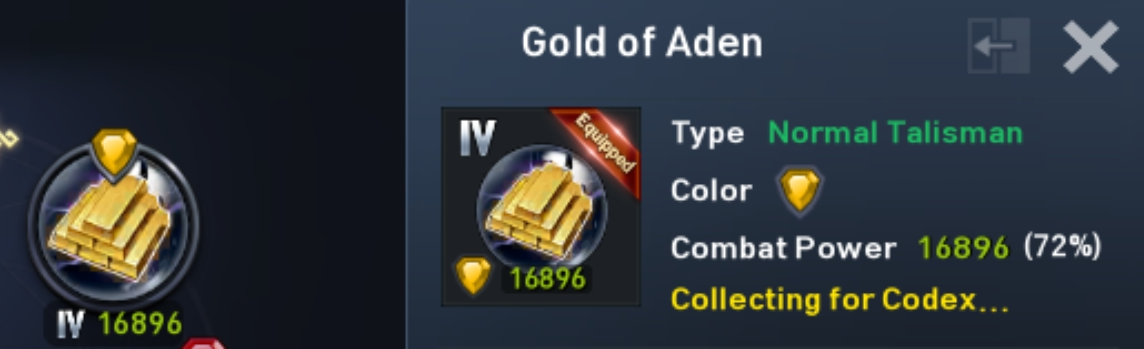
\includegraphics[scale=0.5]{talis3}
\end{center}
Using the above talisman as an example, the listed CP is in the 72nd percentile and it has a green name.
This means that 28\% of Gold of Aden talisman will have more CP and 72\% will have less.

Combinations of colors will apply additional effects, which are unlocked via the combination codex.
Combinations have different tiers of increasing complexity and rarity.
You will need to unlock a combination in order to use it, then you will need to equip the proper combination of colors to activate that combination.

\pagebreak
Note: blue is 'B' and black is 'b'
\begin{center}
\textbf{Normal Combinations}

\begin{tabular}{|c|>{\centering}p{8cm}|m{5cm}|}
	\hline 
	Combination & Effect & Items to Unlock\\ 
	\hline 
	PPP & Evasion & Fairy Wing Fragment\newline History of Avento\\ 
	\hline 
	BBB & Rare Skill Dmg Decrease & Hunter's Token\newline Pixie Wing\\ 
	\hline 
	RRR & Ignore Rare Skill Dmg Decrease & Glory of Conquerors\newline Conqueror's Challenge\\ 
	\hline 
	YYY & Accuracy & Scar of Oren\newline Blessing of Pixies\\ 
	\hline 
	WWW & PVP Crit Dmg Decrease & Fate of Schuttgar\newline Spirit's Dark Flame\\ 
	\hline 
	bbb & Ignore PVP Crit Dmg Decrease & Hope of Avento\newline Shard of Trials\\ 
	\hline 
	BBP & Accuracy & Azure Insignia Orb*\\ 
	\hline 
	RRW & Evasion & Crimson Sun Orb*\\ 
	\hline 
	YYb & Accuracy & Golden Glory Orb*\\ 
	\hline 
	BPP & Crit Rate & Magenta Twilight Orb*\\ 
	\hline 
	RWW & PVP Crit Dmg Decrease & Sacred Power Orb*\\ 
	\hline 
	Ybb & Crit Res & Obsidian Devil Orb*\\ 
	\hline 
\end{tabular} 

*Acquired from Treasure Guard
%\pagebreak

\textbf{High-grade Combinations}
\begin{tabular}{|c|>{\centering}p{8cm}|m{5cm}|}
	\hline 
	Combination & Effect & Items to Unlock \\ 
	\hline 
	BBBRR & Rare Skill Dmg Decrease, Res & Garden Pebble\newline Demon's Trace \\ 
	\hline 
	RRRYY & Ignore Rare Skill Dmg Decrease, Pen & Ancient Bone Shard\newline Marlox's Horn\newline Zaken's Ring \\ 
	\hline 
	YYYPP & Crit Rate, Pen & Fairy Tears\newline Marsha's Fan\newline Dragon Scale Shard \\ 
	\hline 
	PPPWW & PVP Crit Dmg Decrease, Evasion & Freyja's Curs\newline Courage Toke\newline Dragon Claw \\ 
	\hline 
	WWWbb & Crit Res, PVP Crit Dmg Decrease & Sound of Memories\newline Secret of Schuttgart \\ 
	\hline 
	BBbbb & Ignore PVP Crit Dmg Decrease, Accuracy & The Devil's Temptation\newline Memory of Avento \\ 
	\hline 
\end{tabular} 


\textbf{Rare Combinations}

\begin{tabular}{|c|>{\centering}p{8cm}|m{5cm}|}
	\hline 
	Combination & Effect & Items to Unlock \\ 
	\hline 
	PPWWWWW & PVP Crit Dmg Decrease, Evasion, Max MP & Gladiator's Iron Wall Shield\newline Deadman's Chest\newline Warrior's Spirit \\ 
	\hline 
	BBBBBbb & Ignore PVP Crit Dmg Decrease, Accuracy, Max MP & Protection of Wind\newline Gladiator's Blessing \\ 
	\hline 
	BBRRRRR & Rare Skill Dmg Decrease, Res, Evasion & Promise of Pixies\newline Marlox's Claws \\ 
	\hline 
	RRYYYYY & Ignore Rare Skill Dmg Decrease, Pen, Accuracy & Countess's Ring\newline Temptation of Madness\newline Zaken's Eye \\ 
	\hline 
	YYPPPPP & Crit Rate, Pen, Accuracy & Countess's Nails\newline Whisper of Madness\newline Golden Gargoyle Scale \\ 
	\hline 
	WWbbbbb & Crit Res, Res, Evasion & Pledge of Sacrifice\newline Order of Schuttgart \\ 
	\hline 
\end{tabular} 

\pagebreak
\textbf{Heroic Combinations}

\begin{tabular}{|c|>{\centering}p{8cm}|m{5cm}|}
	\hline 
	Combination & Effect & Items to Unlock \\ 
	\hline 
	BBBBBRRW & Rare Skill Dmg Decrease, Res, M. Def, P. Def & Divine Orb Blessing* \\ 
	\hline 
	RRRRRYYb & Ignore Rare Skill Dmg Decrease, Pen, P. Def, M. Def & Starving Destruction Orb* \\ 
	\hline 
	BYYYYYPP & Crit Rate, Ignore PVP Crit Dmg Decrease, P. Def, M. Def & Merciless Rage Orb* \\ 
	\hline 
	RPPPPPWW & PVP Crit DMG Decrease, Res, P. Def, M. Def & Lustrous Silverlight Imprint Orb* \\ 
	\hline 
	YWWWWWbb & Crit Res, Res, P. Def, M. Def & Noble Sacrifice Orb* \\ 
	\hline 
	BBPbbbbb & Ignore PVP Crit Dmg Decrease, Pen, P. Def, M. Def & Fallen Abyss Orb* \\ 
	\hline 
\end{tabular} 

*Dropped from field and world bosses


\end{center}

Talisman may be salvaged for Talisman Essence, which may be used to bind boxes which contain a random talisman.
Talisman essence is dictated by the color of the talisman being salvaged (e.g., purple yields purple essence).
\begin{center}
	\textbf{Talisman Salvage Yields}
\end{center}
\begin{itemize}
	\item IV - 60 Essence
	\item III - 35 Essence
	\item II - 26 Essence
	\item I - 19 Essence
\end{itemize}

\section{Everything Else}

Achievements are a good CP bump but are not very easy to farm.
Take a look through your achievements just to see if there are any easy ones left to do.

Arena is a good source of both CP and red gems.
Resets of arena are 10, 20, 30, 40, and 50 red gems, for a total of 150 red gems.
Ranks 1, 2, and 3 gives 300, 200, and 150 red gems respectively, so if you have any shot of reaching these ranks it is a good idea to spend the gems to reset.
For lower ranks, you will want to keep a budget in mind while doing resets.
The top 100 will give 60 red gems, which allows you to be neutral with up to 3 resets;
the top 1\% and 3\% give 40 and 30, respectively, so it's a good idea to do a few resets if you fall in those ranks.
Remember to hit up Open Siege on Tuesday, Thursday, and Sunday for the extra honor!

For rifts, it isn't a great idea to farm nightmare rifts unless you have an abundance of red gems.
At 200 per run, things can get expensive very quickly, and the CP increase from NM CoBB or AoM is fairly low.
For the others, farm what you can and try to avoid resetting rifts outside of events.

If you find yourself flush with red gems and have no equipment to reroll, resetting SC and doing full resets of arena are a good idea.
You may also want to purchase some agathion boxes, or check out the event shop to see what's available that day.

\pagebreak
\section{General Thoughts}

If you are willing to spend, then spend smart.
Always purchase mounts, as they are usually only available for a short period of time, and avoid buying costumes if you are looking for CP as they provide very little.
The 260 jump-up bundle at \$99.99 is your best buy, as it will give around 100k CP and enough blues to purchase a costume.
The two lower level jump-up bundles are also worth the purchase, but those can't be purchased at level 320+.
Daily item benefits at \$4.99 is also a smart buy if you plan on farming beads, and the 2x rift benefit at \$9.99 is a very good idea if you want to speed up your rift farming.

Do the math on events, and try to plan things out from the start.
Many events require resetting dungeons or rifts a certain number of times, and missing a few days can make it impossible to finish the event.
If there are multiple rewards available, try to prioritize mounts, titles, or other things that may give CP - mats can be obtained at any time!

Show up to sieges, even if you have no opponent or are just rotating a castle.
You will get adena rewards by simply being present when the siege ends.

When you are farming adena in an elite dungeon, try to farm efficiently.
If you have good CP and can kill quickly, then look for areas that do not have many people.
On the other end, if you have low CP and kill slowly, then try to group up and work with other people.
At level 330+, the adena gained from elite mob drops far outweighs the cost of soulshots, so it is smart to use SS while AFK farming to maximize adena and experience gains.

If you find yourself well below acceptable CP for your level - say 400k+ CP below others at your level - then it is a good idea to stop leveling: no fires, no weekly quests, no experience dungeon, no elite dungeon AFKing.
Turn yourself in to a farming machine for cores and other things that can increase your CP but don't require much adena.

To estimate where you stand in terms of CP, take a look at the top CP player on your server.
To keep pace, you can think of things in terms of this inequality, $[CP_{your}]$ \textgreater $\frac{[CP_{top}]}{2}$. Therefore, if the top CP on the server is 4.5 million, then your CP should be higher than 2.25 million in order to keep up with the pace of CP inflation. To be competitive with the top players, you will want this equation to hold true, $[CP_{your}] \geq \frac{2[CP_{top}]}{3}$. Which is the same as saying that you would need at least 3 million CP to compete if the top player has 4.5 million CP.

Honorable Battlefield - commonly known as 3v3 - runs for one hour every Monday, Wednesday, and Friday.
While not directly contributing to your CP, the rewards from 3v3 can be very helpful in your CP growing efforts.
Each match will reward points, which can be used to buy Hero accessories, unconfirmed scrap, and boxes.
At the end of each season, your final league rank (Silver, Gold, Platinum, and so on) will result in a reward box which contains blue diamonds, red diamonds, a title, and some more battlefield points.

Lastly, do not forget about alt characters.
While they do not directly provide CP, your alt characters can provide an increase to your main's primary statistics by up to 5\%. 
In order to achieve this 5\% bump, you will need to have a total of 4 characters (other than your main) with a total of 500 levels.
The easiest way to achieve this is by leveling 4 characters to level 125, which can be done in a few days.
An important note on this is that orcs factor in differently than other races due to their higher starting level.
In short, a level 180 orc counts the same as a level 1 human/elf/dark elf/dwarf, and 1 orc level is the same as 0.5 levels for the other races.
\pagebreak

\section*{Acknowledgements}
Special thanks to my fellow Guild members for giving me idea to write the first version of this back in November of 2018.
I originally wrote this to help our low CP members catch up, and I have tried to keep it updated ever since then.

Thanks to everyone in Horde alliance and F4 alliance for sharing their knowledge and experiences with these systems.

And thanks to everyone that has read this document, I hope you've found it helpful!

Feel free to send me a DM on Discord: Burl\#1908

\nocite{*}
\bibliographystyle{IEEEtran}
\bibliography{LCG.bib}
\end{document}
